% !TeX root = ../document.tex

\chapter{狭义相对论}
\begin{xiti}
	\item 惯性 观者$G$和$G^\prime$相对 速率 为$u=0.6 c$,相遇 时 把 时钟 都 调为 零。用 时空图 讨论:(a) 在$G$所属的惯性参考系看来(以其同时观判断),当$G$钟读数为$\SI{5}{\micro\second} $时,$G^\prime$钟的读数是多少?(b)当$G$钟读数为$\SI{5}{\micro\second} $时,他实际看见$G^\prime$钟的读数是多少?

	\begin{jie}
		如图~\ref{pic-6.1},其中$a$点$G$的固有时为$\tau=\SI{5}{\micro\second}$。

		\begin{figure}[htb!]
			\centering
			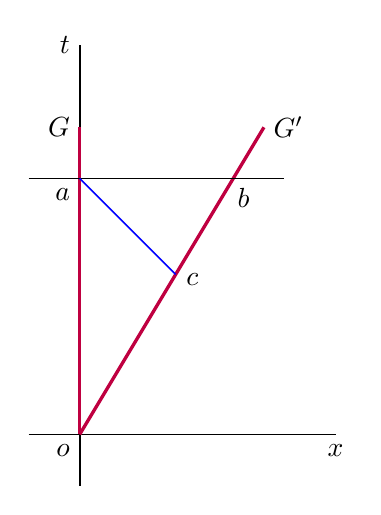
\begin{tikzpicture}[scale=1.3]
			\node[below] (x) at (2.5,0) {$x$};
			\node[left] (t) at (0,3.8) {$t$};
			\node[below left] (O) at (0,0) {$o$};
			\node[left] (G) at (0,3) {$G$};
			\node[right] (g) at (1.8,3) {$G^\prime$};
			\node[below left] (tau) at (0,2.5) {$a$};
			\node[below] (b) at (1.6,2.5) {$b$};
			\node[below] (c) at (1.1,1.6625) {$c$};
			\draw[semithick,\myarrow] (-0.5,0) -- (2.5,0);
			\draw[semithick,\myarrow] (0,-0.5) -- (0,3.8);
			\draw[very thick,purple] (0,0) -- (0,3);
			\draw[very thick,purple] (0,0) -- (1.8,3);
			\draw (-0.5,2.5) -- (2,2.5);
			\draw[semithick,blue,\myarrow] (0.938,1.562) -- (0,2.5);
			\end{tikzpicture}
			\caption{题1解答图}\label{pic-6.1}
		\end{figure}

	    \begin{enumerate}
	    	\item[(a)] 易知 $b$点的$x$坐标为$0.6\tau$,于是 $b$ 点 $G^\prime$ 的固有时为 \[\tau^\prime = \sqrt{1-0.6^2} \tau = 0.8 \tau = \SI{4}{\micro\second}.\]
	    	\item[(b)] 易求得$c$点在${t,x}$坐标系下的坐标为 $\displaystyle \left( \frac{5}{8} \tau ,\frac{3}{8} \tau \right)$\footnote{$t$在前,$x$在后},于是$c$点$G'$的固有时为 \[ \tau^{\prime\prime} = \sqrt{\left(\frac{5}{8}\right)^2-\left(\frac{3}{8}\right)^2} \tau = \frac{\tau}{2} = \SI{2.5}{\micro\second}. \]
	    \end{enumerate}
	\end{jie}

	\item 远方星体以$0.8 c $的速率(匀速直线地)离开我们,我们测得它辐射来的闪光按$5$昼夜的周期变化。用时空图求星上观者测得的闪光周期。

	\begin{jie}
		如图~\ref{pic-6.2},
		\begin{figure}[htb!]
			\centering
			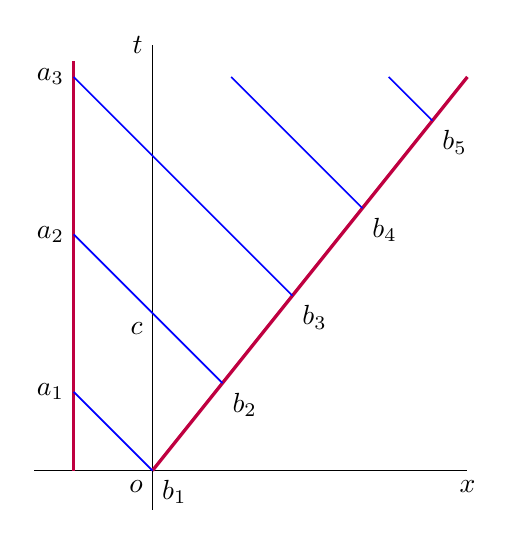
\begin{tikzpicture}
			\node[below] (x) at (5,0) {$x$};
			\node[left] (t) at (1,5.4) {$t$};
			\node[below left] (O) at (1,0) {$o$};
			\node[left] (a1) at (0,1) {$a_1$};
			\node[left] (a2) at (0,3) {$a_2$};
			\node[left] (a3) at (0,5) {$a_3$};
			\node[below right] (b1) at (1,0) {$b_1$};
			\node[below left] (c) at (1,2) {$c$};
			\draw[semithick,\myarrow] (-0.5,0) -- (5,0);
			\draw[semithick,\myarrow] (1,-0.5) -- (1,5.4);
			\draw[very thick,purple] (0,0) -- (0,5.2);
			\draw[very thick,purple] (1,0) -- (5,5);
			\draw[semithick,blue,\myarrow] (1.8889,1.1111) node[below right,black] {$b_2$} -- (0,3);
			\draw[semithick,blue,\myarrow] (1,0) -- (0,1);
			\draw[semithick,blue,\myarrow] (2.7778,2.2222) node[below right,black] {$b_3$} -- (0,5);
			\draw[semithick,blue,\myarrow] (3.6667,3.3333) node[below right,black] {$b_4$} -- (2,5);
			\draw[semithick,blue,\myarrow] (4.5556,4.4444) node[below right,black] {$b_5$} -- (4,5);
			\end{tikzpicture}
			\caption{题2解答图}\label{pic-6.2}
		\end{figure}
	    记$c$点坐标为$\left(\tau,0\right)$,其中$\tau=\SI{5}{\day}$,则可算得$b_2$点坐标为 $\displaystyle \left(\frac{5}{9},\frac{4}{9}\right) \tau$,于是$b_1$到$b_2$星上观者经过的固有时$\displaystyle \tau^{\prime} = \sqrt{5^2-4^2} \frac{\tau}{9} = \frac{\tau}{3} = \frac{5}{3} \,\si{\day}.$
	\end{jie}

	\item 把图~\hyperlink{6-20}{6-20}~的 $oa$ 段和 $oe$ 段线长分别记作 $\tau$ 和 $\tau^\prime$ 。(a) 用两钟的相对速率 $u$ 表出 $\tau^\prime/\tau$ ;(b) 在 $u=0.6c$ 和 $u=0.8c$ 两种情况下求出 $\tau^\prime/\tau$ 的数值。

	\begin{figure}[htb!]
		\centering
		\begin{tikzpicture}
		\draw[very thick,purple] (0,0) node[left,black] {$o$} -- (0,-5);
		\draw[very thick,purple] (0,0) -- (2,-5);
		\node[above left] (a) at (0,-2) {$a$};
		\draw[semithick,domain=-1.732:1.732,variable=\t,range=0:4, smooth] plot ({2*\t},{-2*sqrt(\t*\t+1)});
		\draw[semithick,blue,\myarrow] (1.333,-3.333) node[below right,black] {$e$} -- (0,-2);
		\node (jz) at (-2.15,-3) {\colorbox{white}{校准曲线}};
		\node[above,rotate=90] (c) at (0,-3.5) {$C$钟(观者$G$)};
		\node (cc) at (1,-0.9) {$C'$钟};
		\end{tikzpicture}
		\caption{正文图6-20}\hypertarget{6-20}{}
	\end{figure}

    \begin{jie}
    	\begin{enumerate}
    		\item[(a)] 如图~\ref{pic-6.3},记 $t=of$,
    		\begin{equation}
    		\frac{\tau'}{\tau} = \frac{\sqrt{t^2-u^2 t^2}}{t-ut} = \sqrt{\frac{1+u}{1-u}}.
    		\end{equation}

    		\begin{figure}[htb!]
    			\centering
    			\begin{tikzpicture}
    			\draw[very thick,purple] (0,0) node[left,black] {$o$} -- (0,-5);
    			\draw[very thick,purple] (0,0) -- (2,-5);
    			\node[above left] (a) at (0,-2) {$a$};
    			\draw[semithick,domain=-1.732:1.732,variable=\t,range=0:4, smooth] plot ({2*\t},{-2*sqrt(\t*\t+1)});
    			\draw[semithick,blue,\myarrow] (1.333,-3.333) node[below right,black] {$e$} -- (0,-2);
    			\draw[semithick] (1.333,-3.333) -- (0,-3.333) node[below right] {$f$} ;
    			\node (jz) at (-2.15,-3) {\colorbox{white}{校准曲线}};
    			\node[above,rotate=90] (c) at (0,-3.5) {$C$钟(观者$G$)};
    			\node (cc) at (1,-0.9) {$C'$钟};
    			\end{tikzpicture}
    			\caption{题3解答图}\label{pic-6.3}
    		\end{figure}

    	    \item[(b)] 将 $u=0.6$ 和 $u=0.8$ 代入,分别得 $\dfrac{\tau'}{\tau}$ 为 $2$ 和 $3$。
    	\end{enumerate}
    \end{jie}

    \item 惯性质点 $A,B,C$ 排成一条直线并沿此线相对运动(见~\hyperlink{t5}{图 6.5}),相对速率 $u_{BA}=0.6 c$ , $u_{CA}=0.8 c$ ,$A,B$ 所在惯性系各为 $\mathscr{R}_A$ 和 $\mathscr{R}_B$。设 $\mathscr{R}_B$ 系认为(测得)$C$ 走了 $\SI{60}{m}$,画出时空图并求 $\mathscr{R}_A$ 认为(测得)这一过程的时间。

    \begin{figure}[htb!]
    	\centering
    	\begin{tikzpicture}[scale=1.5]
    	\filldraw (0,0) circle (0.02cm);
    	\filldraw (1,0) circle (0.02cm);
    	\filldraw (2,0) circle (0.02cm);
    	\draw[semithick] (0,0) node[below] {$A$} -- (1,0) node[below] {$B$} -- (2,0) node[below] {$C$} -- (3,0);
    	\draw[thick,-{Latex[length=6pt,width'=0pt 0.4]}] (1,0.15) -- (1.6,0.15);
    	\draw[thick,-{Latex[length=6pt,width'=0pt 0.4]}] (2,0.15) -- (2.8,0.15);
    	\end{tikzpicture}
    	\caption{题4用图}\hypertarget{t5}{}
    \end{figure}

    \begin{jie}
    	如图~\ref{pic-6.4},
    	\begin{figure}[htb!]
    		\centering
    		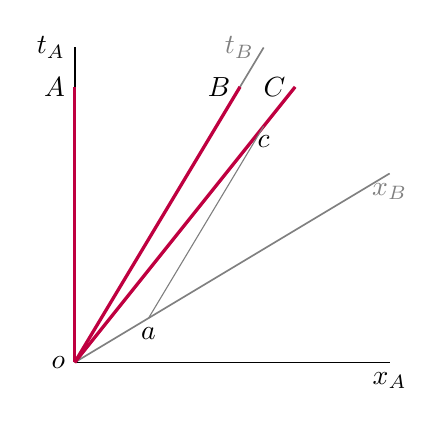
\begin{tikzpicture}
    		\draw[semithick,\myarrow] (0,0) -- (4,0);
			\draw[semithick,\myarrow] (0,0) -- (0,4);
			\draw[semithick,gray,\myarrow] (0,0) -- (2.4,4);
			\draw[semithick,gray,\myarrow] (0,0) -- (4,2.4);
			\node[left] (o) at (0,0) {$o$};
			\node[left] (tA) at (0,4) {$t_A$};
			\node[below] (xA) at (4,0) {$x_A$};
			\node[left,gray] (tB) at (2.4,4) {$t_B$};
			\node[below,gray] (xB) at (4,2.4) {$x_B$};
    		\draw[very thick,purple] (0,0) -- (0,3.5);
    		\draw[very thick,purple] (0,0) -- (2.1,3.5);
			\draw[very thick,purple] (0,0) -- (2.8,3.5);
			\node[left] (A) at (0,3.5) {$A$};
			\node[left] (B) at (2.1,3.5) {$B$};
			\node[left] (C) at (2.8,3.5) {$C$};
			\draw[gray] (0.9375,0.5625) -- (2.4,3);
			\node[below] (c) at (2.4,3) {$c$};
			\node[below] (D) at (0.9375,0.5625) {$a$};
			\end{tikzpicture}
			\caption{题4解答图}\label{pic-6.4}
		\end{figure}
		$oa$ 段长 $\displaystyle l=\SI{60}{\meter}$,则可算得 $a$ 的坐标为 $\displaystyle \left( \frac{3}{4} , \frac{5}{4} \right) l$,由 $ac$ 的斜率为 $\displaystyle \frac{1}{0.6}$,$oc$ 的斜率为 $\displaystyle \frac{1}{0.8}$ 可求得 $c$ 点坐标为 $\displaystyle \left(4,\frac{16}{5}\right) l$,即 $oc$ 在 $\mathscr{R}_A$ 看来的时间为 $\displaystyle \frac{4l}{c} = \frac{240}{299792458} \si{\second}$。
	\end{jie}

	\item $A,B$ 是同一惯性系的两个惯性观者,他们互相发射中子,每一中子以相对速率 $0.6 c$ 离开中子枪。设 $B$ 测得 $B$ 枪的中子发射速率为 $\SI{e4}{s^{-1}}$ (即每秒发射 $10^4$ 个),求 $A$ 所发中子(根据中子自己的标准钟)测得的 $B$ 枪的中子发射率(要求画时空图求解)。

	\begin{jie}
		如图~\ref{pic-6.5},$oa$长为 $\Delta\tau_B$,则由对称性易知 $\displaystyle ob=ab=\frac{\Delta\tau_B}{2}$,则 $bc=0.3\Delta\tau_B$,故算得 $\Delta\tau=ac=0.4\Delta\tau_B$,因此 $A$ 发射的中子测得的 $B$ 的发射率为 $\displaystyle f=\frac{1}{\Delta\tau}=2.5f_B=\SI{2.5e4}{\per\second}$。
		\begin{figure}[htb!]
			\centering
			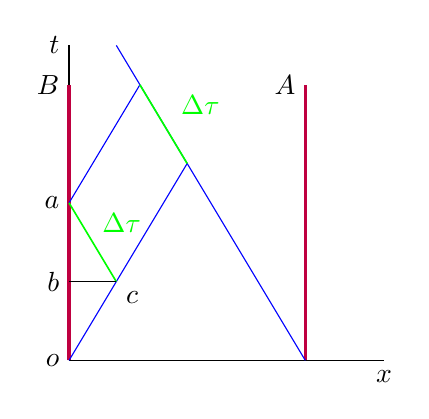
\begin{tikzpicture}
				\draw[semithick,\myarrow] (0,0) -- (0,4);
				\draw[semithick,\myarrow] (0,0) -- (4,0);
				\draw[very thick,purple] (0,0) -- (0,3.5);
				\draw[very thick,purple] (3,0) -- (3,3.5);
				\node[left] (o) at (0,0) {$o$};
				\node[left] (t) at (0,4) {$t$};
				\node[below] (x) at (4,0) {$x$};
				\node[left] (A) at (3,3.5) {$A$};
				\node[left] (B) at (0,3.5) {$B$};
				\draw[blue,\myarrow] (3,0) -- (0.6,4);
				\draw[blue,\myarrow] (0,0) -- (1.5,2.5);
				\draw[blue,\myarrow] (0,2) -- (0.9,3.5);
				\draw[semithick,green] (0.9,3.5) -- (1.5,2.5);
				\draw[semithick,green] (0,2) -- (0.6,1);
				\node[above right,green] (tau) at (1.3,3) {$\Delta \tau$};
				\node[above right,green] (tau2) at (0.3,1.5) {$\Delta \tau$};
				\node[left] (a) at (0,2) {$a$};
				\node[left] (b) at (0,1) {$b$};
				\node[below right] (c) at (0.6,1) {$c$};
				\draw (0,1) -- (0.6,1);
			\end{tikzpicture}
			\caption{题5解答图}\label{pic-6.5}
		\end{figure}
	\end{jie}

	\item 静止 $\mu$ 子的平均寿命为 $\tau_0=\SI{2e-6}{s}$。宇宙线产生的 $\mu$ 子相对于地球以 $0.995c$ 的速率匀速直线下落,用时空图求地球观者测得的(a)$\mu$子的平均寿命;(b)$\mu$子在其平均寿命内所走过的距离。

		\begin{jie}
			如图~\ref{pic-6.6},$ac=\tau_0$,$bc=t$ 为地球看来的平均寿命。则 $ab=0.995t$,有
			\begin{equation*}
				\tau_0=ac=\sqrt{\abs{-t^2+(0.995t)^2}}\approx 0.09987 t,
			\end{equation*}
			故 $t\approx 10.0125 \tau_0 = \SI{2.0025e-5}{\second}$,而走过的距离为 $ab=vt\approx\SI{5.9733}{\kilo\metre}$。
			\begin{figure}[htb!]
				\centering
				\begin{tikzpicture}
					\draw[semithick,\myarrow] (0,0) -- (0,3);
					\draw[semithick,\myarrow] (0,0) -- (4,0);
					\node[left] (o) at (0,0) {$o$};
					\node[left] (t) at (0,3) {$t$};
					\node[below] (x) at (4,0) {$x$};
					\draw[blue,\myarrow] (3,0) -- (1.01,2);
					\draw[very thick,purple] (0,0) -- (0,2.5);
					\draw[gray] (1.01,0) -- (1.01,2);
					\node[below] (a) at (3,0) {$a$};
					\node[below left] (b) at (1.01,0) {$b$};
					\node[left] (c) at (1.01,2) {$c$};
				\end{tikzpicture}
				\caption{图6解答图}\label{pic-6.6}
			\end{figure}
		\end{jie}

	\item 从惯性系 $\mathscr{R}$ 看来(认为,测得),位于某地 $A$ 的两标准钟甲、乙指零时开始以速率 $v=0.6c$ 一同做匀速直线运动,两钟指 $\SI{1}{\second}$ 时到达某地 $B$。甲钟在到达 $B$ 地时立即以速率 $v$ 向 $A$ 地匀速返回,乙钟在 $B$ 地停留 $\SI{1}{\second}$ (按他的钟)后以速率 $v$ 向 $A$ 的匀速返回。另有一丙钟一直呆在 $A$ 地,且当甲、乙离开 $A$ 地时也指零,(a) 画出甲、乙、丙的世界线;(b) 求乙钟返回 $A$ 地时三钟的读数 $\tau_{\text{甲}}$,$\tau_{\text{乙}}$ 和 $\tau_{\text{丙}}$。

		\begin{jie}
			如图~\ref{pic-6.7},设$A$ 地位于 $x=0$,$B$ 地位于 $x=s$。
			\begin{figure}[htb!]
				\centering
				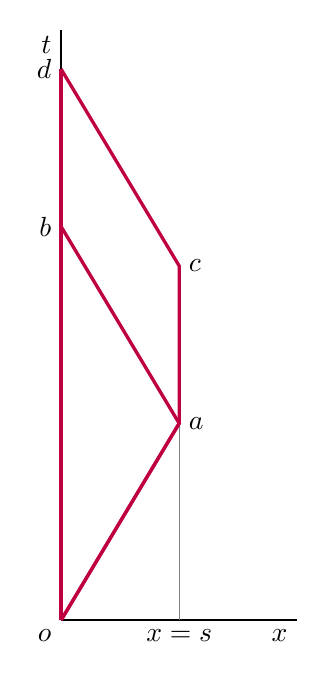
\begin{tikzpicture}
					\draw[semithick,\myarrow] (0,0) -- (0,7.5);
					\draw[semithick,\myarrow] (0,0) -- (3,0);
					\node[below left] (o) at (0,0) {$o$};
					\node[left] (t) at (0,7.3) {$t$};
					\node[below left] (x) at (3,0) {$x$};
					\draw[gray] (1.5,0) -- (1.5,2.5);
					\node[below] (s) at (1.5,0) {$x=s$};
					\draw[very thick,purple] (0,0) -- (1.5,2.5) -- (0,5) -- (0,7);
					\draw[very thick,purple] (0,0) -- (1.5,2.5) -- (1.5,4.5) -- (0,7);
					\draw [very thick,purple] (0,0) -- (0,7);
					\node[right] (a) at (1.5,2.5) {$a$};
					\node[left] (b) at (0,5) {$b$};
					\node[right] (c) at (1.5,4.5) {$c$};
					\node[left] (d) at (0,7) {$d$};
				\end{tikzpicture}
				\caption{题7解答图}\label{pic-6.7}
			\end{figure}
			\begin{enumerate}[label=(\alph*)]
				\item 甲的世界线为 $oabd$;乙的世界线为 $oacd$;丙的世界线为 $obd$。
				\item 由题干知线长 $oa=ac=ab=bd=cd$ 都是 $\tau=\SI{1}{\second}$,故 $\displaystyle \tau_{\text{甲}}=\tau_{\text{乙}}=\SI{3}{\second}$。$a$ 点位于 $\displaystyle \left(\frac{5}{3}s,s\right)$,$\displaystyle oa=\frac{4}{3}s$,故 $\displaystyle s=\frac{3}{4}\tau$,则 $\displaystyle ob=2\times \frac{5}{3}s = \frac{5}{2} \tau$,于是 $\displaystyle \tau_{\text{丙}}=\frac{7}{2}\tau=\SI{3.5}{\second}$。
			\end{enumerate}
		\end{jie}

	\item (单选题)双子 $A$,$B$ 静止于某惯性系 $\mathscr{R}$ 中的同一空间点上。$A$ 从某时刻(此时$A$,$B$ 年龄相等)开始向东以速率 $u$ 相对于惯性系 $\mathscr{R}$ 做惯性运动,一段时间后 $B$ 以速率 $v>u$ 向东追上 $A$,则相遇时 $A$ 的年龄

	\begin{tabularx}{\textwidth}{XXX}
		(1)~比 $B$ 大, & (2)~比 $B$ 小, & (3)~与 $B$ 等。
	\end{tabularx}

		\begin{jie}
			选 (1)。$A$ 走了测地线,而 $B$ 不是测地线。
		\end{jie}

	\item 标准钟 $A$,$B$ 静止于某惯性系中的同一空间点上。$A$ 钟从某时刻开始以速率 $u=0.6c$ 匀速直线飞出,$\SI{2}{\second}$(根据$A$ 钟)后以 $u=0.6c$ 匀速直线返航。已知分手时两钟皆指零。(1) 求重逢时两钟的读数;(2) 当 $A$ 钟指 $\SI{3}{\second}$ 时看见 $B$ 钟指多少?

		\begin{jie}
			\begin{enumerate}
				\item 由 $u=0.6c$ 知 $\displaystyle \gamma=\frac{5}{4}$,故 $\Delta\tau_\text{A}=\SI{2}{\second}$ 对应 $\displaystyle \Delta t=\SI{5/2}{\second}$,由于 $B$ 钟在惯性系中静止,重逢时 $\tau_\text{B}=\SI{5}{\second}$,$\tau_{\text{A}}=\SI{4}{\second}$。
				\item 如图~\ref{pic-6.9},记 $\tau=\SI{2}{\second}$,则 $a$ 的坐标为 $\displaystyle\left( \frac{3}{4} \tau, \frac{5}{4}\tau \right)$,$b$ 的坐标为 $\displaystyle \left( 0,\frac{5}{2} \tau \right)$,$\tau_\text{A}=\SI{3}{\second}$ 的 $c$ 位于 $\displaystyle \left( \frac{3}{8}\tau, \frac{15}{8} \right)$,则可算出 $d$ 位于 $\displaystyle \left( 0,\frac{3}{2}\tau \right)$,故 $c$ 点处 $A$ 看见 $B$ 的读数为 $\displaystyle \frac{3}{2} \tau = \SI{3}{\second}$。
			\end{enumerate}

			\begin{figure}[htb!]
				\centering
				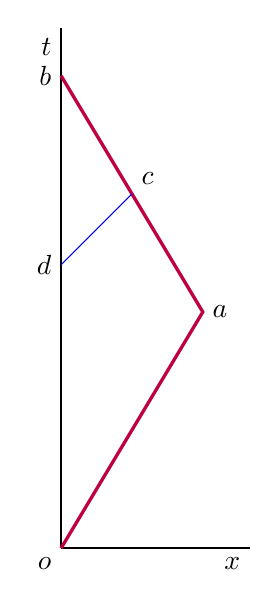
\begin{tikzpicture}[scale=0.6]
					\draw[semithick,\myarrow] (0,0) -- (0,11);
					\draw[semithick,\myarrow] (0,0) -- (4,0);
					\node[below left] (o) at (0,0) {$o$};
					\node[below left] (t) at (0,11) {$t$};
					\node[below left] (x) at (4,0) {$x$};
					\draw[very thick,purple] (0,0) -- (3,5) -- (0,10);
					\node[right] (a) at (3,5) {$a$};
					\node[left] (b) at (0,10) {$b$};
					\node[above right] (c) at (1.5,7.5) {$c$};
					\draw[blue,\myarrow] (0,6) node[left,black]{$d$} -- (1.5,7.5);
				\end{tikzpicture}
				\caption{题9解答图}\label{pic-6.9}
			\end{figure}
		\end{jie}

	\item 地球自转线速率在赤道之值约为每小时 $\SI{1600}{\kilo\metre}$。甲、乙为赤道上的一对孪生子。甲坐飞机以每小时 $\SI{1600}{\kilo\metre}$ 的速率向西绕赤道飞行一圈后回家与乙重逢(忽略地球和太阳引力场的影响。由第7章可知引力的存在对应于时空的弯曲。)。(a) 画出地球表面的世界面和甲、乙的世界线(甲相对于地面的运动抵消了地球自转的效应,所以甲是惯性观者。);(b) 甲与乙中谁更年轻?(c) 两者年龄相差多少?(答:约为$\SI{e-7}{\second}$。)注:本实验已于 1971 年完成,当然不是对人而是对铯原子钟。见\cite{Hafele166}。

		\begin{jie}
			如图~\ref{pic-6.10}。
			\begin{figure}[htb!]
				\centering
				% \begin{tikzpicture}
				% 	\begin{axis}[view={60}{30}]
				% 	\addplot3 [
				% 	mesh,
				% 	z buffer=sort,
				% 	samples=20,
				% 	domain=-1:0,
				% 	y domain=0:2*pi,
				% 	] (
				% 	{cos(deg(y))},
				% 	{sin(deg(y))},
				% 	x
				% 	);
				% 	\end{axis}
				% \end{tikzpicture}
				\begin{tikzpicture}
					\draw (-2,-2) rectangle (2,2);
					\node (emm) at (0,0) {图暂略……};
				\end{tikzpicture}
				\caption{题10解答图}\label{pic-6.10}
			\end{figure}
			\begin{enumerate}[label=(\alph*)]
				\item 233
				\item 乙更年轻。
				\item 以坐标时 $t$ 为参数,乙的世界线切矢模长为
				\begin{equation*}
					\norm{\tensor{\left( \pdv{t} \right)}{^a}} = \sqrt{1-u^2},
				\end{equation*}
				其中 $u$ 是自转的3-速率,则乙经过的线长为
				\begin{equation*}
					\tau = \int_0^T \norm{\tensor{\left( \pdv{t} \right)}{^a}} \dd{t} = \sqrt{1-u^2} T,
				\end{equation*}
				代入 $u$ 和 $T=\SI{1}{\day}$ 知
				\begin{equation*}
					T-\tau=\left( 1- \sqrt{1-u^2} \right) T = \SI{9.49449e-8}{\second}.
				\end{equation*}
			\end{enumerate}
		\end{jie}

	\item 静长 $l=\SI{5}{\metre}$ 的汽车以 $u=0.6c$ 的速率匀速进库,库有坚硬后墙。为简化问题,假定车头撞墙的信息以光速传播,车身任一点接到信息立即停下。(a) 设司库测得在车头撞墙的同时车尾的钟 $\mathrm{C_w}$ 指零,求车尾“获悉”车头撞墙这一信息时 $\mathrm{C_w}$ 的读数;(b) 求车完全停下后的静长 $\hat{l}$;(c) 用 $u$ 表示新旧静长比 $\hat{l}/l$。

		\begin{jie}
			如图~\ref{pic-6.11},
			\begin{figure}[htb!]
				\centering
				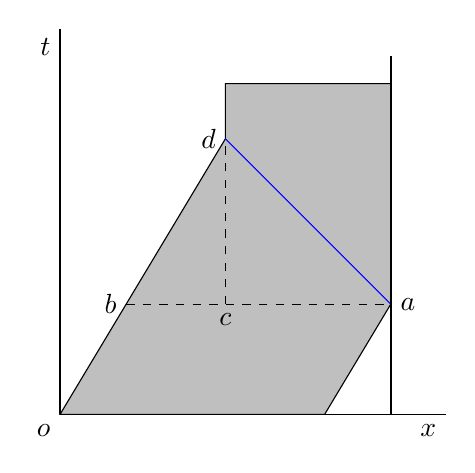
\begin{tikzpicture}[scale=0.7]
					\draw[semithick,\myarrow] (0,0) -- (0,7);
					\draw[semithick,\myarrow] (0,0) -- (7,0);
					\node[below left] (o) at (0,0) {$o$};
					\node[below left] (t) at (0,7) {$t$};
					\node[below left] (x) at (7,0) {$x$};
					\filldraw[fill=gray!50!white] (0,0) -- (3,5) -- (3,6) -- (6,6) -- (6,2) -- (4.8,0) -- cycle;
					\draw[blue,\myarrow] (6,2) node[right,black]{$a$} -- (3,5);
					\draw[thick] (6,0) -- (6,6.5);
					\draw[dashed] (1.2,2) node[left]{$b$} -- (6,2);
					\draw[dashed] (3,2) node[below]{$c$} -- (3,5) node[left]{$d$};
				\end{tikzpicture}
				\caption{题11解答图}\label{pic-6.11}
			\end{figure}
			$ac=cd=\hat{l}$,则 $bc=u\hat{l}$,$ab=(1+u)\hat{l}$,而由尺缩公式知 $ab=\sqrt{1-u^2}l$,故
			\begin{equation*}
				(1+u)\hat{l} = \sqrt{1-u^2} l, \implies \hat{l} = \sqrt{\frac{1-u}{1+u}}l,
			\end{equation*}
			则
			\begin{equation*}
				bd=\sqrt{cd^2-bc^2} = \sqrt{1-u^2} \hat{l} = l,
			\end{equation*}
			故
			\begin{enumerate}[label=(\alph*)]
				\item $\mathrm{C_w}$ 的读数为 $bd=l$,恢复$c$ 即 $\displaystyle \frac{l}{c}=\frac{5}{299792458}\si{\second} \approx \SI{1.66782e-8}{\second}$。
				\item 代入 $u=0.6c$ 知 $\displaystyle \hat{l}=\frac{l}{2}=\SI{2.5}{\metre}$。
				\item $\displaystyle \frac{\hat{l}}{l} = \sqrt{\frac{1-u}{1+u}}$。
			\end{enumerate}
		\end{jie}

	\item 试证命题 6-3-4.

	\begin{zm}
		命题6-3-4如下
		\begin{yl}{Thm}
			质点世界线上各点的4加速 $\tensor{A}{^a}$ 与 4 速 $\tensor{U}{^a}$ 正交,即 $\tensor{A}{^a} \tensor{U}{_a} = \tensor{\eta}{_a_b} \tensor{A}{^a} \tensor{U}{^b} =0$。
		\end{yl}
		\begin{yl}{Prf}
			\begin{equation*}
				\begin{split}
					\tensor{U}{_a}\tensor{A}{^a} &= \tensor{U}{_a} \tensor{U}{^b} \Partial{b} \tensor{U}{^a} \\
					&= \frac{1}{2} \tensor{U}{^b} \Partial{b} \left( \tensor{U}{_a} \tensor{U}{^a} \right)\\
					&=0.
				\end{split}
			\end{equation*}
		\end{yl}
	\end{zm}

	\item 设观者世界线为 $t\sim x$ 面内的双曲线 $G$ (见\hyperlink{t6}{图 6-43}),图中 $K$ 为已知,$\tensor{A}{^a}$ 为观者的 4 加速,求 $\tensor{A}{^a} \tensor{A}{_a}$(结论是 $\tensor{A}{^a} \tensor{A}{_a}$ 为常数,因此 $G$ 称为匀加速运动观者\footnote{或称 Rindler 观者——笔者注}。请注意这指的是4加速。)

	\begin{figure}[htb]
		\centering
		\begin{tikzpicture}[decoration={brace,amplitude=6},scale=0.7]
			\draw[semithick,\myarrow] (-3.5,0) -- (3.5,0);
			\draw[semithick,\myarrow] (0,-3.5) -- (0,3.5);
			\node[left] (t) at (0,3.5) {$t$};
			\node[below] (x) at (3.5,0) {$x$};
			\draw[semithick,loosely dash dot] (-3,-3) -- (3,3);
			\draw[semithick,loosely dash dot] (-3,3) -- (3,-3);
			\draw[domain=-1.732:1.732,variable=\t,range=0:4, smooth,thick] plot ({1.5*sqrt(\t*\t+1)},{1.5*\t});
			\node (G) at (2.5,1.5) {$G$};
			\node (K) at (0.75,-0.7) {\colorbox{white}{$K$}};
			\draw[decorate] (1.5,0) -- (0,0);
		\end{tikzpicture}
		\caption{原书图 6-43}\hypertarget{t6}{}
	\end{figure}

	\begin{jie}
		由图知此双曲线的参数为 $a=b=K$ ,可写出双曲线方程为
		\begin{equation*}
			x^2-t^2=K^2,
		\end{equation*}
		两边对固有时求导,
		\begin{gather*}
			2x \dv{x}{\tau} - 2t \dv{t}{\tau} = 0,\\
			\dv{x}{\tau} = \frac{t}{x} \dv{t}{\tau},
		\end{gather*}
		而
		\begin{equation*}
			\begin{split}
				\tensor{Z}{^a} &= \dv{t}{\tau} \tensor{\left(\pdv{t}\right)}{^a} + \dv{x}{\tau} \tensor{\left(\pdv{x}\right)}{^a}
			\end{split}
		\end{equation*}
		是归一的,则
		\begin{equation*}
			\begin{split}
				\left(\dv{x}{\tau} \right)^2 - \left( \dv{t}{\tau} \right)^2 &= \left[ \left(\frac{t}{x}\right)^2 - 1 \right] \left( \dv{t}{\tau} \right)^2\\
				&= - \left( \frac{K}{x} \dv{t}{\tau} \right)^2\\
				&= -1,
			\end{split}
		\end{equation*}
		\begin{equation*}
			\implies \frac{1}{x} \dv{t}{\tau} = \frac{1}{t} \dv{x}{\tau} = \frac{1}{K},
		\end{equation*}
		于是4速又可改写为
		\begin{equation*}
			\tensor{Z}{^a} = \frac{1}{K} \left[ x \tensor{\left(\pdv{t}\right)}{^a} + t \tensor{\left(\pdv{x}\right)}{^a} \right],
		\end{equation*}
		故
		\begin{equation*}
			\begin{split}
				\tensor{A}{^a} &= \dv{\tensor{Z}{^a}}{\tau}\\
				&= \frac{1}{K} \left[ \dv{x}{\tau} \tensor{\left(\pdv{t}\right)}{^a} + \dv{t}{\tau} \tensor{\left(\pdv{x}\right)}{^a} \right]\\
				&= \frac{1}{K^2} \left[ t \tensor{\left(\pdv{t}\right)}{^a} + x \tensor{\left(\pdv{x}\right)}{^a} \right],\\
				\tensor{A}{_a} \tensor{A}{^a} &= \frac{1}{K^4} \left( x^2 - t^2 \right)\\
				&= \frac{1}{K^2}.
			\end{split}
		\end{equation*}
	\end{jie}

	\item 试证命题6-6-2.

	\begin{zm}
		命题6-6-2如下
		\begin{yl}{Thm}
			设惯性系 $\mathscr{R}$ 和 $\mathscr{R}^\prime$ 由洛伦兹变换
			\begin{equation*}
				t = \gamma \left( t^\prime + v x^\prime \right) \qc x = \gamma \left( x^\prime + v t^\prime \right) \qc y = y^\prime \qc z = z^\prime
			\end{equation*}
			相联系,则两者测同一电磁场 $\tensor{F}{_a_b}$ 所得值 $\left( \myvec{E},\myvec{B} \right)$ 和 $\left( \myvec{E}^\prime , \myvec{B}^\prime \right)$ 有如下关系:
			\begin{align*}
				E_1^\prime &= E_1, & E_2^\prime &= \gamma \left( E_2 - v B_3 \right), & E_3^\prime &= \gamma \left( E_3 + v B_2 \right);\\
				B_1^\prime &= B_1, & B_2^\prime &= \gamma \left( B_2 + v E_3 \right), & B_3^\prime &= \gamma \left( B_3 - v E_2 \right).
			\end{align*}
		\end{yl}
		\begin{yl}{Prf}
			记矩阵 $\Lambda$ 为
			\begin{equation*}
				\left[ \tensor{\Lambda}{^\mu_\nu} \right] = \left[ \pdv{x^\mu}{x^{\prime\nu}} \right] = \mqty( \mqty{ \gamma & \gamma v \\ \gamma v & \gamma }  & \mqty{\zmat{2}{2}} \\ \mqty{\zmat{2}{2}} & \mqty{\imat{2}} ),
			\end{equation*}
			则易知
			\begin{equation*}
				\left[ \tensor{\left(\Lambda^{-1}\right)}{^\mu_\nu} \right] = \left[ \pdv{x^{\prime\mu}}{x^{\nu}} \right] = \mqty( \mqty{ \gamma & - \gamma v \\ - \gamma v & \gamma }  & \mqty{\zmat{2}{2}} \\ \mqty{\zmat{2}{2}} & \mqty{\imat{2}} ),
			\end{equation*}
			而根据张量变换律
			\begin{equation*}
				\begin{split}
					\tensor{{F^\prime}}{^\mu_\nu} &= \pdv{x^{\prime\mu}}{x^\sigma} \pdv{x^\rho}{x^{\prime\nu}} \tensor{F}{^\sigma_\rho}\\
					&= \tensor{\left(\Lambda^{-1}\right)}{^\mu_\sigma} \tensor{F}{^\sigma_\rho} \tensor{\Lambda}{^\rho_\nu},
				\end{split}
			\end{equation*}
			于是有矩阵等式
			\begin{equation*}
				\left[F^\prime\right] = \Lambda^{-1} \left[F\right] \Lambda,
			\end{equation*}
			其中 $\left[F\right]$ 表示 $\tensor{F}{^\mu_\nu}$ 排成的矩阵
			\begin{equation*}
				\left[F\right] = \mqty( 0 & E_1 & E_2 & E_3 \\ E_1 & 0 & B_3 & -B_2 \\ E_2 & -B_3 & 0 & B_1 \\ E_3 & B_2 & -B_1 & 0 ),
			\end{equation*}
			于是经过简单的矩阵乘法算得
			\begin{equation*}
				\left[ F^\prime \right] = \mqty( 0 & E_1 & \gamma \left( E_2 - v B_3 \right) & \gamma \left( E_3 + v B_2 \right) \\ E_1 & 0 & \gamma \left( B_3 - v E_2 \right) & - \gamma \left( B_2 + v E_3 \right) \\ \gamma \left( E_2 - v B_3 \right) & - \gamma \left( B_3 - v E_2 \right) & 0 & B_1 \\ \gamma \left( E_3 + v B_2 \right) & \gamma \left( B_2 + v E_3 \right) & -B_1 & 0 ),
			\end{equation*}
			可以直接读出
			\begin{align*}
				E_1^\prime &= E_1, & E_2^\prime &= \gamma \left( E_2 - v B_3 \right), & E_3^\prime &= \gamma \left( E_3 + v B_2 \right);\\
				B_1^\prime &= B_1, & B_2^\prime &= \gamma \left( B_2 + v E_3 \right), & B_3^\prime &= \gamma \left( B_3 - v E_2 \right).
			\end{align*}
		\end{yl}
	\end{zm}

	\item 设瞬时观者测 $\tensor{F}{_a_b}$ 所得电场和磁场分别为 $\tensor{E}{^a}$ 和 $\tensor{B}{^a}$(也记为 $\myvec{E}$ 和 $\myvec{B}$),试证:
	\begin{enumerate}[label=(\alph*)]
		\item $\tensor{F}{_a_b} \tensor{F}{^a^b} = 2 \left( B^2 - E^2 \right)$,
		\item $\tensor{F}{_a_b} \tensor[^*]{F}{^a^b} = 4 \myvec{E} \vdot \myvec{B}$。提示:可利用惯性坐标基底把 $\tensor{F}{_a_b} \tensor[^*]{F}{^a^b}$ 写成分量表达式。
	\end{enumerate}
	注:本题表明,虽然 $\myvec{E}$ 和 $\myvec{B}$ 都是观者依赖的,$B^2-E^2$ 和 $\myvec{E} \vdot \myvec{B}$ 却同观者无关。事实上,由 $\tensor{F}{_a_b}$ 能构造的独立的不变量只有这两个。

		\begin{zm}
			我表示并不想用分量……用分量的话矩阵相乘求迹,看官自行计算。还是几何语言看着舒服,虽然看着计算更长……
			\begin{Lemma}
				\label{lemma-6.15}
				对任意参考系有分解式
				\begin{equation*}
					\tensor{F}{_a_b} = \tensor{Z}{_a} \tensor{E}{_b} - \tensor{Z}{_b} \tensor{E}{_a} + \tensor{\varepsilon}{_a_b_c} \tensor{B}{^c},
				\end{equation*}
				其中
				\begin{equation*}
					\tensor{\varepsilon}{_a_b_c} = \tensor{\varepsilon}{_d_a_b_c} \tensor{Z}{^d}
				\end{equation*}
				是“空间体元”(因为 $\tensor{Z}{^a}$ 未必是某超曲面法矢故加引号)。
			\end{Lemma}
			\begin{Proof}
				由
				\begin{equation*}
					\tensor{B}{_a} = - \tensor[^*]{F}{_a_b} \tensor{Z}{^b} = - \frac{1}{2} \tensor{\varepsilon}{_a_b_c_d} \tensor{F}{^c^d} \tensor{Z}{^b} = \frac{1}{2} \tensor{\varepsilon}{_a_c_d} \tensor{F}{^c^d},
				\end{equation*}
				知
				\begin{equation*}
					\tensor{\varepsilon}{_a_b_c} \tensor{B}{^c} = \frac{1}{2} \tensor{\varepsilon}{_a_b_c} \tensor{\varepsilon}{^c^d^e} \tensor{F}{_d_e} = \tensor{h}{^{d}_{[a}} \tensor{h}{^{e}_{b]}} \tensor{F}{_d_e} = \tensor{h}{^{d}_a} \tensor{h}{^{e}_b} \tensor{F}{_d_e},
				\end{equation*}
				其中 $\tensor{h}{^a^b} = \tensor{\delta}{^a_b} + \tensor{Z}{^a} \tensor{Z}{_b}$ 是空间投影,而即使 $\tensor{Z}{^a}$ 不是某超曲面法矢,也可以通过展开计算证明有 $\tensor{\varepsilon}{_a_b_c} \tensor{\varepsilon}{^c^d^e} = 2\tensor{h}{^{d}_{[a}} \tensor{h}{^{e}_{b]}}$。进一步展开得
				\begin{equation*}
					\tensor{\varepsilon}{_a_b_c} \tensor{B}{^c} = \left( \tensor{\delta}{^d_a} + \tensor{Z}{^d} \tensor{Z}{_a} \right) \left( \tensor{\delta}{^e_b} + \tensor{Z}{^e} \tensor{Z}{_b} \right) \tensor{F}{_d_e} = \tensor{F}{_a_b} - \tensor{Z}{_a} \tensor{E}{_b} + \tensor{Z}{_b} \tensor{E}{_a}.
				\end{equation*}
			\end{Proof}
			由引理直接计算:
			\begin{enumerate}[label=(\alph*)]
				\item
				\begin{equation*}
					\begin{split}
						\tensor{F}{_a_b} \tensor{F}{^a^b} &= \left( \tensor{Z}{_a} \tensor{E}{_b} - \tensor{Z}{_b} \tensor{E}{_a} + \tensor{\varepsilon}{_a_b_c} \tensor{B}{^c} \right) \left( \tensor{Z}{^a} \tensor{E}{^b} - \tensor{Z}{^b} \tensor{E}{^a} + \tensor{\varepsilon}{^a^b^d} \tensor{B}{_d} \right)\\
						&= -E^2 - E^2 + \tensor{\varepsilon}{_a_b_c} \tensor{\varepsilon}{^a^b^d} \tensor{B}{^c} \tensor{B}{_d}\\
						&= 2 \left( B^2 - E^2 \right).
					\end{split}
				\end{equation*}
				\item 易算得
				\begin{equation}
					\begin{split}
						\tensor[^*]{F}{_a_b} &= \frac{1}{2} \tensor{\varepsilon}{_a_b_c_d} \tensor{F}{^c^d}\\
						&= \frac{1}{2} \tensor{\varepsilon}{_a_b_c_d} \left( \tensor{Z}{^c} \tensor{E}{^d} - \tensor{Z}{^d} \tensor{E}{^c} + \tensor{\varepsilon}{^c^d^e} \tensor{B}{_e} \right)\\
						&= \tensor{Z}{_b}\tensor{B}{_a} - \tensor{Z}{_a} \tensor{B}{_b} + \tensor{\varepsilon}{_a_b_c} \tensor{E}{^c},\label{eq-*F}
					\end{split}
				\end{equation}
				故
				\begin{equation*}
					\begin{split}
						\tensor{F}{_a_b} \tensor[^*]{F}{^a^b} &=  \left( \tensor{Z}{_a} \tensor{E}{_b} - \tensor{Z}{_b} \tensor{E}{_a} + \tensor{\varepsilon}{_a_b_c} \tensor{B}{^c} \right) \left( \tensor{Z}{^b}\tensor{B}{^a} - \tensor{Z}{^a} \tensor{B}{^b} + \tensor{\varepsilon}{^a^b^d} \tensor{E}{_d} \right)\\
						&= \tensor{E}{_b} \tensor{E}{^b} + \tensor{E}{_a} \tensor{B}{^a} + \tensor{\varepsilon}{_a_b_c} \tensor{\varepsilon}{^a^b^d} \tensor{B}{^c} \tensor{E}{_d}\\
						&= 4 \tensor{E}{_a} \tensor{B}{^a}.
					\end{split}
				\end{equation*}
			\end{enumerate}
		\end{zm}

	\item 试证命题 6-6-5 (只需证后两个麦氏方程)。

		\begin{zm}
			命题 6-6-5 如下
			\begin{Proposition}
				对任一惯性系 $\left\{ t,x,y,z\right\}$,由式 (6-6-10)、(6-6-11)\footnote{正文 (6-6-10) 为 $\tensor{\partial}{^a} \tensor{F}{_a_b} = - 4\pi \tensor{J}{_b}$,正文 (6-6-11) 为 $\tensor{\partial}{_{[a}} \tensor{F}{_{bc]}} = 0$。} 可导出 3 维麦氏方程
				\begin{align*}
					(a) \nabla \vdot \myvec{E} &= 4\pi \rho, & (b) \nabla \cross \myvec{E} &= - \pdv{\myvec{B}}{t},\\
					(c) \nabla \vdot \myvec{B} &= 0 , & (d) \nabla \cross \myvec{B} &= 4\pi \myvec{j} + \pdvt{\myvec{E}}.
				\end{align*}
				其中第一、四式对应于式 (6-6-10),第二、三式对应于式 (6-6-11)。
			\end{Proposition}
			证明如下:式 (c):
			\begin{equation*}
				\nabla\vdot\myvec{B} = \tensor{\partial}{_a} \tensor{B}{^a} = - \tensor{\partial}{_a} \tensor[^*]{F}{^a^b} \tensor{Z}{_b} = - \frac{1}{2} \tensor{\varepsilon}{^a^b^c^d} \tensor{Z}{_b} \tensor{\partial}{_a} \tensor{F}{_c_d} = 0,
			\end{equation*}
			式 (d):
			\begin{equation*}
				\begin{split}
					\tensor{\hat{\varepsilon}}{^a^b^c} \tensor{\partial}{_b} \tensor{B}{_c} &= - \tensor{Z}{_d} \tensor{\varepsilon}{^d^a^b^c} \tensor{\partial}{_b} \tensor[^*]{F}{_c_e} \tensor{Z}{^e}\\
					&= \frac{1}{2} \tensor{Z}{_d} \tensor{Z}{^e} \tensor{\varepsilon}{^c^d^a^b} \tensor{\varepsilon}{_c_e_m_n} \tensor{\partial}{_b} \tensor{F}{^m^n}\\
					&= - \frac{3!}{2} \tensor{Z}{_d} \tensor{Z}{^e} \tensor{\delta}{^d_{[e}} \tensor{\delta}{^a_m} \tensor{\delta}{^b_{n]}} \tensor{\partial}{_b} \tensor{F}{^m^n}\\
					&= - \tensor{Z}{_d} \tensor{Z}{^e} \left( \tensor{\delta}{^d_e} \tensor{\delta}{^a_m} \tensor{\delta}{^b_n} + \tensor{\delta}{^d_m} \tensor{\delta}{^a_n} \tensor{\delta}{^b_e} + \tensor{\delta}{^d_n} \tensor{\delta}{^a_e} \tensor{\delta}{^b_m} \right) \tensor{\partial}{_b} \tensor{F}{^m^n}\\
					&= \tensor{\partial}{_b} \tensor{F}{^a^b} - \tensor{Z}{^b} \tensor{Z}{_d} \tensor{\partial}{_b} \tensor{F}{^d^a} - \tensor{Z}{_d} \tensor{Z}{^a} \tensor{\partial}{_b} \tensor{F}{^b^d}\\
					&= -\tensor{h}{^a_d} \tensor{\partial}{_b} \tensor{F}{^b^d} + \tensor{Z}{^b} \tensor{\partial}{_b} \tensor{E}{^a}\\
					&= 4\pi \tensor{j}{^a} + \partial_t \tensor{E}{^a}.
				\end{split}
			\end{equation*}
			\begin{tcolorbox}[breakable,title=补充,fonttitle=\normalfont\bfseries]
				笔者认为由引理~\ref{lemma-6.15} 计算更优雅,且4维麦氏方程与3维麦氏方程的等价性非常显然。计算如下:

				由引理~\ref{lemma-6.15} 知
				% \begin{equation*}
				% 	\begin{split}
				% 		\tensor{\partial}{_a} \tensor{F}{_b_c} &= \tensor{\partial}{_a} \left( \tensor{Z}{_b} \tensor{E}{_c} - \tensor{Z}{_c} \tensor{E}{_b} + \tensor{\varepsilon}{_b_c_d} \tensor{B}{^d} \right)
				% 	\end{split}
				% \end{equation*}
				% 知
				% \begin{equation*}
				% 	\tensor{\partial}{^a} \tensor{F}{_a_c} = \partial_t \tensor{E}{_c}
				% \end{equation*}
				\begin{equation*}
					\begin{split}
						\tensor{\partial}{^a} \tensor{F}{_a_b} &= \tensor{\partial}{^a} \left( \tensor{Z}{_a} \tensor{E}{_b} - \tensor{Z}{_b} \tensor{E}{_a} + \tensor{\varepsilon}{_a_b_c} \tensor{B}{^c} \right) = {\color{blue}\Partial{t} \tensor{E}{_b}} {\color{green} {}-\tensor{Z}{_b} \tensor{\partial}{^a} \tensor{E}{_a}} {\color{blue}{}-\tensor{\varepsilon}{_b_a_c} \tensor{\partial}{^a} \tensor{B}{^c}}\\
						&= -4\pi\tensor{J}{_b} = {\color{green} -4\pi \rho \tensor{Z}{_b}} {\color{blue}{}-4\pi\tensor{j}{_b}},
					\end{split}
				\end{equation*}
				其中蓝色表示空间张量,绿色表示正比于 $\tensor{Z}{_a}$ 的时间部分,故可直接读出
				\begin{equation*}
					\tensor{\partial}{_a} \tensor{E}{^a} = 4\pi \rho , \qq{或} \nabla \vdot \myvec{E} = 4 \pi \rho,
				\end{equation*}
				以及
				\begin{equation*}
					\Partial{t} \tensor{E}{_a} - \tensor{\varepsilon}{_a_b_c} \tensor{\partial}{^b} \tensor{B}{^c} = - 4\pi \tensor{j}{_a}, \qq{或} \nabla\cross \myvec{B} = 4\pi \myvec{j} + \pdvt{\myvec{E}},
				\end{equation*}
				同样地,由
				\begin{equation*}
					\begin{split}
						\tensor{\varepsilon}{^a^b^c^d} \tensor{\partial}{_{b}} \tensor{F}{_{cd}} &= \tensor{\varepsilon}{^a^b^c^d} \tensor{Z}{_c}\tensor{\partial}{_{b}}  \tensor{E}{_d} + \tensor{\varepsilon}{^a^b^c^d} \tensor{\varepsilon}{_f_c_d_e} \tensor{Z}{^f} \tensor{\partial}{_b} \tensor{B}{^e}\\
						&= \tensor{\varepsilon}{^a^b^d} \tensor{\partial}{_b} \tensor{E}{_d} - \left( \tensor{\delta}{^a_f} \tensor{\delta}{^b_e}- \tensor{\delta}{^a_e} \tensor{\delta}{^b_f} \right) \tensor{Z}{^f} \tensor{\partial}{_b} \tensor{B}{^e}\\
						&= {\color{blue} \tensor{\varepsilon}{^a^b^d} \tensor{\partial}{_b} \tensor{E}{_d}} {\color{green} {}-\tensor{Z}{^a}\tensor{\partial}{_b} \tensor{B}{^b}} {\color{blue}{}+\Partial{t} \tensor{B}{^a}}\\
						&=0
					\end{split}
				\end{equation*}
				直接读出
				\begin{equation*}
					\tensor{\partial}{_a} \tensor{B}{^a} = 0 \qq{或} \nabla \vdot \myvec{B} = 0,
				\end{equation*}
				及
				\begin{equation*}
					\tensor{\varepsilon}{^a^b^d} \tensor{\partial}{_b} \tensor{E}{_d} + \Partial{t} \tensor{B}{^a} = 0 \qq{或} \nabla \cross \myvec{B} = - \pdvt{\myvec{B}}.
				\end{equation*}
				这样不仅很快推出了四条三维麦氏方程,而且显然四条三麦氏方程包含了两条四维方程的所有信息。此外,以上计算容易推广到非惯性系乃至弯曲时空任意参考系的一般情况,看官读过中册 \S 14.1 后不妨尝试。
			\end{tcolorbox}
		\end{zm}

	\item 试证瞬时观者测得的电磁场能量密度和3动量密度分别为 $\tensor{T}{_0_0} = \left( E^2 + B^2 \right)/8\pi$ 和 $\tensor{w}{_i} = - \tensor{T}{_i_0} = \tensor{\left( \myvec{E} \cross \myvec{B} \right)}{_i}/4\pi$,$i=1,2,3$。提示:用 $\tensor{F}{_a_b}$ 的对称表达式 (6-6-28')\footnote{正文(6-6-28')为$\displaystyle\tensor{T}{_a_b} = \frac{1}{8\pi} \left( \tensor{F}{_a_c} \tensor{F}{_b^c} + \tensor[^*]{F}{_a_c} \tensor[^*]{F}{_b^c} \right)$。} 可简化 $\tensor{T}{_0_0}$ 的计算。

		\begin{zm}
			% 吐槽:明明用6-6-28和6-6-28'没啥区别嘛……反正 $\tensor{F}{_a_b} \tensor{F}{^a^b}$ 在 15 题已经算过了……
			直接计算
			\begin{equation*}
				\begin{split}
					\tensor{T}{_0_0} &= \tensor{T}{_a_b} \tensor{Z}{^a} \tensor{Z}{^b}\\
					&= \frac{1}{8\pi} \tensor{Z}{^a} \left( \tensor{F}{_a_c} \tensor{F}{_b^c} + \tensor[^*]{F}{_a_c} \tensor[^*]{F}{_b^c} \right) \tensor{Z}{^b}\\
					&= \frac{1}{8\pi} \left( E^2 + B^2 \right),
				\end{split}
			\end{equation*}
			而
			\begin{equation*}
				\begin{split}
					\tensor{w}{_a} &= - \tensor{h}{^b_a} \tensor{Z}{^c} \tensor{T}{_b_c}\\
					&= - \frac{1}{4\pi} \tensor{h}{^b_a} \tensor{Z}{^c} \left( \tensor{F}{_b_d} \tensor{F}{_c^d} - \frac{1}{4} \tensor{F}{_d_e} \tensor{F}{^d^e} \tensor{\eta}{_b_c} \right)\\
					&= \frac{1}{4\pi} \tensor{h}{^b_a} \tensor{E}{^d} \tensor{F}{_b_d}\\
					&= \frac{1}{4\pi} \tensor{\varepsilon}{_a_d_e} \tensor{E}{^d} \tensor{B}{^e},
				\end{split}
			\end{equation*}
			其中最后一个等号用了引理~\ref{lemma-6.15},此式即三维语言的
			\begin{equation*}
				\myvec{w} = \frac{1}{4\pi} \myvec{E} \cross \myvec{B}.
			\end{equation*}

			\begin{tcolorbox}[breakable,title=补充,fonttitle=\normalfont\bfseries]
				由引理~\ref{lemma-6.15},容易直接把 $\tensor{T}{_a_b}$ 算出来。首先,
				\begin{equation*}
					\begin{split}
						\tensor{F}{_a_c} \tensor{F}{_b^c} &= \left( \tensor{Z}{_a} \tensor{E}{_c} - \tensor{Z}{_c} \tensor{E}{_a} + \tensor{\varepsilon}{_a_c_d} \tensor{B}{^d} \right) \left( \tensor{Z}{_b} \tensor{E}{^c} - \tensor{Z}{^c} \tensor{E}{_b} + \tensor{\varepsilon}{_b^c^e} \tensor{B}{_e} \right)\\
						&= E^2 \tensor{Z}{_a} \tensor{Z}{_b} + \tensor{Z}{_a} \tensor{\varepsilon}{_b_c_e} \tensor{E}{^c} \tensor{B}{^e} - \tensor{E}{_a} \tensor{E}{_b} + \tensor{Z}{_b} \tensor{\varepsilon}{_a_c_d} \tensor{E}{^c} \tensor{B}{^d} + B^2 \tensor{\delta}{_a_b} - \tensor{B}{_a} \tensor{B}{_b}\\
						&= E^2 \tensor{Z}{_a} \tensor{Z}{_b} + 2\tensor{Z}{_{(a}} \tensor{\varepsilon}{_{b)}_c_e} \tensor{E}{^c} \tensor{B}{^e} + B^2 \tensor{\delta}{_a_b} - \tensor{E}{_a} \tensor{E}{_b} - \tensor{B}{_a} \tensor{B}{_b},
					\end{split}
				\end{equation*}
				由~\eqref{eq-*F} 知 $*$ 运算的效果为
				\begin{equation*}
					\tensor{E}{_a} \mapsto - \tensor{B}{_a} \qc \tensor{B}{_a} \mapsto \tensor{E}{_a},
				\end{equation*}
				故直接写出
				\begin{equation*}
					\begin{split}
						\tensor[^*]{F}{_a_c} \tensor[^*]{F}{_b^c} &= B^2 \tensor{Z}{_a} \tensor{Z}{_b} - 2\tensor{Z}{_{(a}} \tensor{\varepsilon}{_{b)}_c_e} \tensor{B}{^c} \tensor{E}{^e} + E^2 \tensor{\delta}{_a_b} - \tensor{B}{_a} \tensor{B}{_b} - \tensor{E}{_a} \tensor{E}{_b}\\
						&= B^2 \tensor{Z}{_a} \tensor{Z}{_b} + 2\tensor{Z}{_{(a}} \tensor{\varepsilon}{_{b)}_c_e} \tensor{E}{^c} \tensor{B}{^e} + E^2 \tensor{\delta}{_a_b} - \tensor{E}{_a} \tensor{E}{_b} - \tensor{B}{_a} \tensor{B}{_b},
					\end{split}
				\end{equation*}
				故
				\begin{equation*}
					\begin{split}
						\tensor{T}{_a_b} &= \frac{1}{8\pi} \left( \tensor{F}{_a_c} \tensor{F}{_b^c} + \tensor[^*]{F}{_a_c} \tensor[^*]{F}{_b^c} \right)\\
						&= \frac{1}{8\pi} \Big[ {\color{green} \left( E^2 + B^2 \right) \tensor{Z}{_a} \tensor{Z}{_b}} + {\color{orange} 4 \tensor{Z}{_{(a}} \tensor{\varepsilon}{_{b)}_c_d} \tensor{E}{^c} \tensor{B}{^d}} \\
						&\qquad\qquad {}+ {\color{blue} \left( E^2 + B^2 \right) \tensor{\delta}{_a_b} - 2 \tensor{E}{_a} \tensor{E}{_b} - 2 \tensor{B}{_a} \tensor{B}{_b}} \Big],
					\end{split}
				\end{equation*}
				容易读出能量密度
				\begin{equation*}
					\varepsilon = \tensor{Z}{^a} \tensor{Z}{^b} \tensor{T}{_a_b} = \frac{1}{8\pi} \left( E^2 + B^2 \right),
				\end{equation*}
				3动量密度或玻印亭矢量
				\begin{equation*}
					\tensor{w}{_a} = - \tensor{h}{^b_a} \tensor{Z}{^c} \tensor{T}{_b_c} = \frac{1}{4\pi} \tensor{\varepsilon}{_a_c_d} \tensor{E}{^c} \tensor{B}{^d},
				\end{equation*}
				及应力张量,或麦克斯韦张量
				\begin{equation*}
					\tensor{s}{_a_b} = \tensor{h}{^c_a} \tensor{h}{^d_b} \tensor{T}{_c_d} = \frac{1}{4\pi} \left[ \frac{1}{2} \left( E^2 + B^2 \right) \tensor{\delta}{_a_b} - \tensor{E}{_a} \tensor{E}{_b} - \tensor{B}{_a} \tensor{B}{_b} \right].
				\end{equation*}
			\end{tcolorbox}
		\end{zm}

	\item (a) 试证 4 电流密度为 $\tensor{J}{^a}$ 的电磁场 $\tensor{F}{_a_b}$ 的能动张量 $\tensor{T}{_a_b}$ 满足 $\tensor{\partial}{^a} \tensor{T}{_a_b} = - \tensor{F}{_b_c} \tensor{J}{^c}$(由此可知当 $\tensor{J}{^a}=0$ 时有 $\tensor{\partial}{^a} \tensor{T}{_a_b} = 0$);(b) 试证上式在惯性系中的时间分量反映能量守恒,即\cite{guo1995} 40 页式(6.2);空间分量反映3动量守恒,即郭书220页式(7.6)。提示:用4洛伦兹力表达式(6-6-20)\footnote{正文式 (6-6-20) 为 $\tensor{F}{^a} = q \tensor{F}{^a_b} \tensor{U}{^b}$。} 把 $\tensor{F}{_b_c} \tensor{J}{^c}$ 改写为洛伦兹力密度。

		\begin{zm}
			\begin{enumerate}[label=(\alph*)]
				\item 先计算
				\begin{equation*}
					\begin{split}
						\tensor{\partial}{^a} \left( \tensor{F}{_a_c} \tensor{F}{_b^c} \right) &= \tensor{F}{_b_c} \tensor{\partial}{_a} \tensor{F}{^a^c} + \tensor{F}{^a^c} \tensor{\partial}{_a} \tensor{F}{_b_c}\\
						&= - 4\pi \tensor{F}{_b_c} \tensor{J}{^c} + \tensor{F}{^a^c} \tensor{\partial}{_a} \tensor{F}{_b_c},
					\end{split}
				\end{equation*}
				注意到
				\begin{equation*}
					\tensor{\partial}{^a} \tensor[^*]{F}{_a_b} = \frac{1}{2} \tensor{\varepsilon}{_a_b_c_d} \tensor{\partial}{^a} \tensor{F}{^c^d} = 0,
				\end{equation*}
				有
				\begin{equation*}
					\begin{split}
						\tensor{\partial}{^a} \left( \tensor[^*]{F}{_a_c} \tensor[^*]{F}{_b^c} \right) &= \tensor[^*]{F}{^a^c} \tensor{\partial}{_a} \tensor[^*]{F}{_b_c}\\
						&= \frac{1}{4} \tensor{\varepsilon}{^a^c^d^e} \tensor{\varepsilon}{_b_c_m_n} \tensor{F}{_d_e} \tensor{\partial}{_a} \tensor{F}{^m^n}\\
						&= - \frac{3!}{4} \tensor{\delta}{^a_{[b}} \tensor{\delta}{^d_m} \tensor{\delta}{^e_{n]}} \tensor{F}{_d_e} \tensor{\partial}{_a} \tensor{F}{^m^n}\\
						&= - \frac{1}{2} \left( \tensor{F}{_d_e} \tensor{\partial}{_b} \tensor{F}{^d^e} + \tensor{F}{_d_b} \tensor{\partial}{_a} \tensor{F}{^a^d} + \tensor{F}{_b_e} \tensor{\partial}{_a} \tensor{F}{^e^a} \right)\\
						&= - \frac{1}{2} \tensor{F}{_a_c} \tensor{\partial}{_b} \tensor{F}{^a^c} + 2 \pi \tensor{F}{_d_b} \tensor{J}{^d} - 2\pi \tensor{F}{_b_e} \tensor{J}{^e}\\
						&= - 4 \pi \tensor{F}{_b_c} \tensor{J}{^c} - \frac{1}{2} \tensor{F}{^a^c} \tensor{\partial}{_b} \tensor{F}{_a_c},
					\end{split}
				\end{equation*}
				故
				\begin{equation*}
					\begin{split}
						\tensor{\partial}{^a} \tensor{T}{_a_b} &= \frac{1}{8\pi} \tensor{\partial}{^a} \left( \tensor{F}{_a_c} \tensor{F}{_b^c} + \tensor[^*]{F}{_a_c} \tensor[^*]{F}{_b^c} \right)\\
						&= - \tensor{F}{_b_c} \tensor{J}{^c} + \frac{1}{8\pi} \left( \tensor{F}{^a^c} \tensor{\partial}{_a} \tensor{F}{_b_c} - \frac{1}{2} \tensor{F}{^a^c} \tensor{\partial}{_b} \tensor{F}{_a_c} \right)\\
						&= - \tensor{F}{_b_c} \tensor{J}{^c} + \frac{1}{16\pi} \tensor{F}{^a^c} \left( \tensor{\partial}{_a} \tensor{F}{_b_c} + \tensor{\partial}{_c} \tensor{F}{_a_b} + \tensor{\partial}{_b} \tensor{F}{_c_a} \right)\\
						&= - \tensor{F}{_b_c} \tensor{J}{^c}.
					\end{split}
				\end{equation*}
				\item 向时间方向投影:
				\begin{equation*}
					\begin{split}
						&\tensor{\partial}{^a} \left( \tensor{T}{_a_b} \tensor{Z}{^b} \right) = \tensor{\partial}{^a} \left( -\varepsilon \tensor{Z}{_a} - \tensor{w}{_a} \right)\\
						={}& - \tensor{Z}{^b} \tensor{F}{_b_c} \tensor{J}{^c} = \tensor{E}{_c} \tensor{j}{^c},
					\end{split}
				\end{equation*}
				即
				\begin{equation*}
					\Partial{t} \varepsilon + \nabla \vdot \myvec{w} + \myvec{E} \vdot \myvec{j} = 0,
				\end{equation*}
				对形如 $(t_1,t_2) \times \Sigma$ 的时空区域积分,左边前两项的积分为 $t_2-t_1$ 时间内 $\Sigma$ 内场的能量增加量,第三项积分为对电荷做功,即电荷能量的增加量,故能量守恒。

				向空间投影:
				\begin{equation*}
					\begin{split}
						&\tensor{h}{^b_a} \tensor{\partial}{^c} \tensor{T}{_c_b} = -\tensor{\partial}{^t} \tensor{w}{_a} + \tensor{\partial}{^c} \tensor{s}{_c_a}=\tensor{\partial}{_t} \tensor{w}{_a} + \tensor{\partial}{^c} \tensor{s}{_c_a}\\
						={}& -\tensor{h}{^b_a} \tensor{F}{_b} = -\tensor{f}{_a},
					\end{split}
				\end{equation*}
				即
				\begin{equation*}
					\Partial{t} \tensor{w}{^i} + \Partial{j} \tensor{s}{^j^i} + \tensor{f}{^i} = 0,
				\end{equation*}
				对形如 $(t_1,t_2) \times \Sigma$ 的时空区域积分,左边前两项的积分为 $t_2-t_1$ 时间内 $\Sigma$ 内场的冲量增加量,第三项积分为对电荷所做冲量,即电荷动量的增加量,故动量守恒。
			\end{enumerate}
		\end{zm}

	\item 试证式 (6-6-29)\footnote{正文式 (6-6-29) 为 $\tensor{A}{_a} = - \phi \tensor{(\dd{t})}{_a} + \tensor{a}{_a}$。} 中的 $\tensor{a}{^a}$ 和 $\phi$ 满足 $\myvec{B} = \nabla \cross \myvec{a}$ 和 $\myvec{E} = -\nabla \phi - \pdv*{\myvec{a}}{t}$,因而的确是电动力学中的3矢势和标势。

		\begin{zm}
			由 $\tensor{A}{_a} = \phi \tensor{Z}{_a} + \tensor{a}{_a}$ 得
			\begin{equation*}
				\begin{split}
					\tensor{\partial}{_{a}} \tensor{A}{_b} &= \tensor{\delta}{^c_a} \tensor{\partial}{_c} \tensor{A}{_b}\\
					&= \left( - \tensor{Z}{_a} \tensor{\partial}{_t} + \tensor{\hat{\partial}}{_a} \right) \left( \phi \tensor{Z}{_b} + \tensor{a}{_b} \right)\\
					&= - \tensor{Z}{_a} \tensor{Z}{_b} \Partial{t} \phi - \tensor{Z}{_a} \Partial{t} \tensor{a}{_b} + \tensor{Z}{_b} \tensor{\hat{\partial}}{_a} \phi + \tensor{\hat{\partial}}{_a} \tensor{a}{_b},
				\end{split}
			\end{equation*}
			故
			\begin{equation*}
				\begin{split}
					\tensor{F}{_a_b} &= 2 \tensor{\partial}{_{[a}} \tensor{A}{_{b]}}\\
					&= - 2\tensor{Z}{_{[a}} \tensor{\partial}{_t} \tensor{a}{_{b]}} - 2\tensor{Z}{_{[a}} \tensor{\hat{\partial}}{_{b]}} \phi +2 \tensor{\hat{\partial}}{_{[a}} \tensor{a}{_{b]}}\\
					&= - 2\tensor{Z}{_{[a}} \tensor{\partial}{_t} \tensor{a}{_{b]}} - 2\tensor{Z}{_{[a}} \tensor{\hat{\partial}}{_{b]}} \phi + \tensor{\varepsilon}{_e_a_b} \tensor{\varepsilon}{^e^c^d} \tensor{\hat{\partial}}{_c} \tensor{a}{_d},
				\end{split}
			\end{equation*}
			与引理~\ref{lemma-6.15} 对比,即知
			\begin{equation*}
				\tensor{E}{^a} = - \Partial{t} \tensor{a}{^a} - \tensor{\hat{\partial}}{^a} \phi \qq{或} \myvec{E} = - \pdvt{\myvec{a}} - \nabla \phi,
			\end{equation*}
			及
			\begin{equation*}
				\tensor{B}{^a} = \tensor{\varepsilon}{^a^b^c} \tensor{\hat{\partial}}{_b} \tensor{a}{_c} \qq{或} \myvec{B} = \nabla \cross \myvec{a}.
			\end{equation*}
		\end{zm}

	\item 在选读 6-1-1 中,(a) 试证 $\Nabla{a} \tensor{\left( \dd{t} \right)}{_b} = 0$,其中 $t$ 为绝对时间,$\Nabla{a}$ 为牛顿时空的导数算符【提示:从式(5-7-2)\footnote{正文式(5-7-2) 为 $\displaystyle \tensor{\left( \pdv{x^\tau} \right)}{^b} \Nabla{b} \tensor{\left( \pdv{x^\mu} \right)}{^a} = \ChristoffelSymbol{\sigma}{\mu}{\tau} \tensor{\left( \pdv{x^\sigma} \right)}{^a}$。}出发。】;(b) 设 $\tensor{w}{^a}$ 为空间矢量(即切于绝对同时面的矢量),$\tensor{v}{^a}$ 为任一4维矢量,试证 $\tensor{v}{^a} \Nabla{a} \tensor{w}{^b}$ 仍为空间矢量【提示:注意$\Nabla{a} t$ 是绝对同时面的法余矢。】。

		\begin{zm}
			\begin{enumerate}[label=(\alph*)]
				\item 由 (5-7-2) 得
				\begin{equation*}
					\begin{split}
						\Nabla{\mu} \tensor{\left( \dd{t} \right)}{_\nu} &= \tensor{\left( \pdv{x^\mu} \right)}{^a} \tensor{\left( \pdv{x^\nu} \right)}{^b} \Nabla{a} \tensor{\left( \dd{t} \right)}{_b}\\
						&= - \tensor{\left( \dd{t} \right)}{_b} \tensor{\left( \pdv{x^\mu} \right)}{^a} \Nabla{a} \tensor{\left( \pdv{x^\nu} \right)}{^b}\\
						&= - \tensor{\left( \dd{t} \right)}{_b} \ChristoffelSymbol{\sigma}{\mu}{\nu} \tensor{\left( \pdv{x^\sigma} \right)}{^b}\\
						&= - \ChristoffelSymbol{0}{\mu}{\nu},
					\end{split}
				\end{equation*}
				由 $\ChristoffelSymbol{\mu}{\nu}{\sigma}$ 在选定特定坐标系下的特殊形式,上式为零。
				\item 由(a) 知 $\Nabla{a} \Nabla{b} t =0$,故
				\begin{equation*}
					\tensor{v}{^a} \left( \Nabla{a} \tensor{w}{^b} \right) \Nabla{b} t = \tensor{v}{^a} \Nabla{a} \left( \tensor{w}{^b} \Nabla{b} t \right) - \tensor{v}{^a} \tensor{w}{^b} \Nabla{a} \Nabla{b} t = 0,
				\end{equation*}
				故 $\tensor{v}{^a} \Nabla{a} \tensor{w}{^b}$ 是空间矢量。
			\end{enumerate}
		\end{zm}

\end{xiti}
